\documentclass{article}

\usepackage{microtype}
\usepackage{graphicx}
\usepackage{subcaption}
\usepackage{booktabs}
\usepackage{multirow}
\usepackage{hyperref}
\newcommand{\theHalgorithm}{\arabic{algorithm}}
\usepackage{icml2026}
\usepackage{amsmath}
\usepackage{amssymb}
\usepackage{mathtools}
\usepackage[capitalize,noabbrev]{cleveref}

\icmltitlerunning{SHIFT-Guard for Burst-Sampled Industrial Time Series}

\begin{document}

\twocolumn[
\icmltitle{SHIFT-Guard: Separating Operating-Condition Shift from Fault Evidence\\
in Burst-Sampled Industrial Time Series}

\begin{icmlauthorlist}
  \icmlauthor{Anonymous Authors}{anon}
\end{icmlauthorlist}
\icmlaffiliation{anon}{Anonymous Institution}
\icmlcorrespondingauthor{Anonymous Authors}{anonymous@example.com}
\icmlkeywords{time-series anomaly detection, predictive maintenance, distribution shift, process monitoring, conformal calibration}
\vskip 0.3in
]

\printAffiliationsAndNotice{}

\begin{abstract}
Industrial anomaly detectors can appear accurate while exploiting acquisition regimes, calendar shifts, or highly overlapping evaluation windows rather than equipment faults. We study a hydraulic press pump dataset containing three vibration/current channels, 20,000 normal samples, and only 600 anomalous samples collected on a different day in short acquisition bursts. We introduce SHIFT-Guard, an evaluation and triage pipeline that constructs gap-safe windows, calibrates only on normal temporal blocks, separates shift and fault evidence into four operational states, and selects models by worst-block false alarms before average discrimination. Across five normal-block folds, the selected Isolation Forest obtains $0.949$ mean F1 and $0.994$ average precision over three seeds while limiting the worst held-out block to two alarm events; models with F1 up to $0.979$ are rejected because they produce five alarms on a normal block. Stress tests, feature ablations, and counterfactual channel repair show that temporal-shape features are more important than amplitude and that current-channel dropout is the selected model's most consequential tested failure mode. The study also demonstrates why burst-level calibration, point-adjustment-free metrics, and explicit limitations are necessary when a nominally large industrial dataset contains only one anomalous record.
\end{abstract}

\section{Introduction}

Time-series anomaly detection (TSAD) is often evaluated as a ranking problem, but a deployed predictive-maintenance system is an alarm policy. Its cost is determined not only by average discrimination, but also by false alarms during unseen normal operating regimes, repeated alerts from overlapping windows, and whether the system confuses sensor/acquisition changes with equipment faults. These concerns are acute in small industrial datasets, where thousands of samples may represent only a few minutes of observation and a single recorded failure.

Evaluation choices can dominate apparent performance. Point adjustment can promote one detected sample into credit for an entire anomalous interval and may make weak scores appear competitive \cite{kim2022rigorous}. Point-wise precision and recall also fail to express existence, overlap, and fragmentation of temporal ranges \cite{tatbul2018precision}. Large benchmark studies further show that data defects and protocol choices can reverse model rankings, and that simple statistical models remain strong competitors \cite{liu2024elephant}. Meanwhile, a normal state absent from training can create systematic false positives under distribution shift \cite{kim2024newnormals}.

We address these issues in a three-channel hydraulic pump dataset from a manufacturing-data competition. The nominally normal and anomalous files are separated by five days, all labels are constant within each file, and acquisition consists of short bursts separated by gaps. Thus, the observed difference can be decomposed only conceptually as
\begin{equation}
\text{observed shift}=\text{fault}+\text{operation}+\text{date/DAQ}+\text{noise},
\end{equation}
and the available data do not identify these terms causally.

Our contribution is therefore a risk-controlled experimental design rather than a claim of universal state-of-the-art accuracy:
\begin{itemize}
  \item We construct windows strictly within acquisition bursts and use five-fold blocked normal validation with separate train, calibration, and normal-test blocks.
  \item We compare five normal-only detectors under one threshold and alarm protocol, without point adjustment, and choose lexicographically by worst-block alarm events, mean alarm events, recall, and average precision.
  \item We define separate fault and shift scores and map them to Green, Yellow-S, Yellow-F, and Red states. The scores are operationally distinct but are not claimed to be statistically independent.
  \item We audit sensor/acquisition perturbations, window length, alarm persistence, feature groups, empirical calibration, and counterfactual channel repair, exposing both gains and failure modes.
\end{itemize}

\section{Related Work}

\paragraph{Reliable TSAD evaluation.}
Range-aware evaluation recognizes that a time interval is not a bag of independent points \cite{tatbul2018precision}. Kim et al.\ show that point adjustment can severely inflate performance \cite{kim2022rigorous}; we therefore report raw window metrics and explicitly merged alarm events. The recent TSB-AD study emphasizes data quality, consistent evaluation, and strong simple baselines \cite{liu2024elephant}. Our protocol adds a manufacturing-specific requirement: every contiguous normal operating block must serve as a held-out regime.

\paragraph{Industrial process monitoring.}
Multivariate projection methods exploit correlated process variables for monitoring and diagnosis \cite{macgregor1995process}. Dynamic PCA augments the observation space with lagged measurements and monitors score-space and residual-space deviations \cite{ku1995dynamic}. We compare both PCA-MSPC and a window-normalized dynamic PCA against a raw range rule, shrinkage Mahalanobis distance, and Isolation Forest \cite{liu2008isolation}. A recurrent reconstruction model is a standard alternative for multi-sensor anomaly detection \cite{malhotra2016lstm}; however, we do not mix a prior, differently split LSTM run into the frozen comparison.

\paragraph{Shift, calibration, and diagnosis.}
Unseen ``new normals'' can degrade unsupervised TSAD \cite{kim2024newnormals}. We do not automatically adapt on test data because fault and normal-shift labels are unavailable; instead, shift evidence triggers quarantine. Conformal scores provide a common scale for heterogeneous detectors \cite{ishimtsev2017conformal}, but ordinary guarantees require exchangeability, which overlapping time windows violate. Time-series conformal methods explicitly relax or adapt to this setting \cite{zaffran2022adaptive,xu2023sequential}. We use empirical $p$-values as calibrated risk ranks and audit them by burst, not as guaranteed posterior probabilities. Finally, process-monitoring contributions can smear across correlated variables; reconstruction-based contribution analysis motivates our counterfactual repair check \cite{alcala2009reconstruction}.

\section{Data and Evaluation Unit}

\subsection{Dataset Audit}

The data contain timestamped measurements from two vibration channels (AI0 and AI1) and one current channel (AI2). The normal file has 20,000 samples from 12 July 2022; the anomalous file has 600 samples from 17 July 2022. The median within-burst interval is 0.1~s, but the files contain long gaps. We begin a new burst when consecutive timestamps differ by more than 0.5~s. This yields 599 normal and 21 anomalous bursts, with a maximum length of 50 samples. Observed acquisition time is 2,000~s normal and 60~s anomalous, although normal wall-clock span is 4,615.8~s.

\begin{table}[t]
\caption{Audited dataset structure. ``Windows'' uses the frozen length $w=10$ and stride one, never crossing a burst boundary.}
\label{tab:data}
\centering
\small
\setlength{\tabcolsep}{3.5pt}
\begin{tabular}{lrrrr}
\toprule
Source & Samples & Bursts & Windows & Obs. time \\
\midrule
Normal & 20,000 & 599 & 14,871 & 2,000 s \\
Anomalous & 600 & 21 & 428 & 60 s \\
\bottomrule
\end{tabular}
\end{table}

The dataset supports anomaly discrimination but not early-failure prediction: every anomalous-file row has the same positive label, no onset time is given, and the file is one calendar record. We consequently treat 21 bursts as acquisition units, not as 21 independent physical failures. Calendar date is never used as a feature.

\subsection{Gap-Safe Windows and Features}

For a burst $b$ with samples $\mathbf{x}_{b,1:T_b}\in\mathbb{R}^3$, we create stride-one windows $\mathbf{X}_{b,t}=\mathbf{x}_{b,t:t+w-1}$ only if all $w=10$ samples lie inside $b$. Each window produces 38 features in five groups:
\begin{itemize}
  \item amplitude (A): standard deviation, RMS, peak-to-peak, and MAD per channel;
  \item shape (S): lag-1/2 autocorrelation, zero-crossing rate, and difference MAD per channel;
  \item relation (R): signed/absolute AI0--AI1 correlation and their standard-deviation ratio;
  \item offset (O): mean, median, and mean absolute value per channel;
  \item acquisition (Q): fractional burst position and burst length.
\end{itemize}
Q is used only by the shift model; fault candidates use raw windows or A/S/R/O subsets.

\section{SHIFT-Guard}

\subsection{Candidate Detectors}

All detectors learn from normal data only. B0 measures the largest robustly scaled excursion beyond training minima/maxima. B1 is an Isolation Forest with 300 trees, 256 samples per tree, a 10--90\% robust scaler, and no anomaly prevalence injected through \texttt{contamination}. M1 uses Ledoit--Wolf shrinkage Mahalanobis distance over S+R. M2 applies PCA-MSPC to A+S+R+O, retains 95\% training variance, and scores the maximum of robustly standardized Hotelling $T^2$ and SPE. M3 z-normalizes each channel within a raw window, flattens its temporal lags, and applies the same PCA-MSPC score. This normalization intentionally suppresses amplitude evidence.

\subsection{Blocked Normal Validation}

We split normal bursts chronologically into five contiguous blocks without cutting a burst. In fold $k$, three blocks train detector and scaler parameters, one block calibrates the threshold, and the remaining block measures normal false alarms. Roles rotate so every block is tested once. The anomalous file is scored in every fold only after model and threshold fitting. Because it remains the same single record, fold-to-fold anomalous scores are repeated robustness views, not independent failures.

For calibration scores $s_1,\ldots,s_n$, the empirical normality rank is
\begin{equation}
p(x)=\frac{1+\sum_{i=1}^{n}\mathbb{1}[s_i\geq s(x)]}{n+1},
\label{eq:pvalue}
\end{equation}
and the alarm threshold is the higher empirical 0.995 quantile. We call $1-p(x)$ a \emph{risk rank}, not a posterior probability. We audit window scores (C0), burst maxima (C1), and burst 95th percentiles (C2). C1/C2 have only 99--113 calibration bursts, so their minimum attainable $p$ exceeds 0.005; zero burst-level rejections at this $\alpha$ are a resolution limit, not evidence of exact coverage.

\subsection{Alarm Policy and Shift/Fault Triage}

A raw exceedance starts an alarm after $k=3$ consecutive above-threshold windows in the same burst and closes it after three consecutive non-exceedances. Alarms never bridge acquisition gaps. We report window precision, recall, F1, MCC, AUROC and AP; normal false-positive windows; merged alarm count; alarms per observed hour; a Poisson 95\% upper rate; and anomalous-burst detection.

After selection, the fault score is the chosen detector. A separate robust Mahalanobis model on A+O+Q forms the shift score. Each is converted using \cref{eq:pvalue}. With $\alpha=0.005$, their flags define four states: Green (neither), Yellow-S (shift only), Yellow-F (fault only), and Red (both). Feature overlap means this is an operational evidence decomposition, not an identifiable causal factorization.

\section{Experiments}

\subsection{Selection Rule and Reproducibility}

Before inspecting results, we fixed a lexicographic selection rule: minimize worst held-out normal-block alarm events, then mean alarm events, then maximize recall and AP. A candidate must also improve over B0. This makes the low-data deployment risk explicit: a detector with perfect anomaly recall is not automatically preferred if one normal regime causes an alarm storm. Stochastic B1 is evaluated at seeds 42, 1337, and 2026 (15 fold-runs); deterministic candidates use seed 42 (five fold-runs). The complete full-mode run takes 29.249~s on a laptop CPU (AMD Ryzen AI 7 PRO 350, 8 cores/16 threads, 27.6~GB RAM).

\subsection{Stress and Sensitivity Tests}

We freeze thresholds before perturbing anomalous windows. The 22 stresses comprise common gains $\{0.5,0.8,1.2,1.5,2.0\}$; offsets $\{-2,-1,+1,+2\}$ training standard deviations; polarity reversal of each vibration channel; Gaussian noise at 1, 5, and 10\%; timestamp jitter from 0.1 to 5~ms; and dropout of each channel. We also vary $w\in\{5,10,20\}$, alarm persistence $k\in\{1,3,5\}$, and remove each A/S/R/O feature group. Window and ablation sensitivity use seed 42 and are reported as diagnostics rather than a post-hoc model replacement.

\section{Results}

\subsection{Predictive Performance Versus False Alarms}

\begin{table*}[t]
\caption{Frozen-protocol comparison. B1 values average three seeds; other models are deterministic five-fold results. Selection prioritizes the maximum number of merged alarms on any held-out normal block (Worst alarms), not F1 alone.}
\label{tab:main}
\centering
\small
\begin{tabular}{lrrrrrrr}
\toprule
Model & Precision & Recall & F1 & AP & FPR & Mean alarms & Worst alarms \\
\midrule
B0 Range & .967 & .533 & .687 & .598 & .0029 & .80 & 2 \\
\textbf{B1 Isolation Forest} & \textbf{.966} & \textbf{.936} & \textbf{.949} & \textbf{.994} & \textbf{.0049} & \textbf{.93} & \textbf{2} \\
M3 Dynamic PCA & .958 & .976 & .967 & .997 & .0061 & 1.00 & 3 \\
M1 Mahalanobis & .959 & 1.000 & .979 & 1.000 & .0063 & 1.40 & 5 \\
M2 PCA-MSPC & .959 & 1.000 & .979 & 1.000 & .0061 & 1.60 & 5 \\
\bottomrule
\end{tabular}
\end{table*}

\Cref{tab:main} illustrates the central selection conflict. M1 and M2 detect every anomalous window and attain F1 near 0.979, but each produces five merged alarms in its worst normal block. B1 keeps B0's worst-block budget of two events while increasing F1 from 0.687 to 0.949 and AP from 0.598 to 0.994. It is therefore selected by the frozen rule. Across B1's 15 runs, mean anomalous-burst detection is 0.925. The mean false-alarm rate is 8.27 per observed acquisition hour; this apparently large rate follows from only 0.56~h of total normal acquisition and should not be extrapolated to a shift-length guarantee.

\begin{figure}[t]
\centering
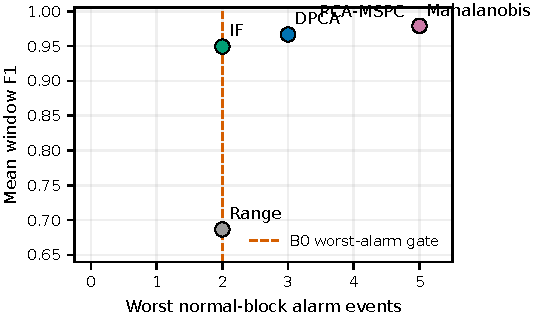
\includegraphics[width=\columnwidth]{figures/selection_tradeoff.pdf}
\caption{Mean F1 versus worst-block merged alarms. The dashed line is the B0 gate. B1 is selected although three alternatives have higher mean F1.}
\label{fig:selection}
\end{figure}

\subsection{Sensitivity and Feature Evidence}

Window length 20 reaches F1 0.984, versus 0.955 at the frozen $w=10$ and 0.818 at $w=5$ (seed 42). We do not promote $w=20$ after observing these results: it delays a decision, excludes more short bursts, and would make the main comparison post hoc. Removing amplitude features improves F1 to 0.974, whereas removing temporal-shape features reduces it to 0.827 and raises worst-block window FPR from 0.0099 to 0.0445. This supports the claim that local dynamics, rather than magnitude alone, carry the most stable fault evidence in this record. It does not prove a physical failure mechanism.

\begin{figure*}[t]
\centering
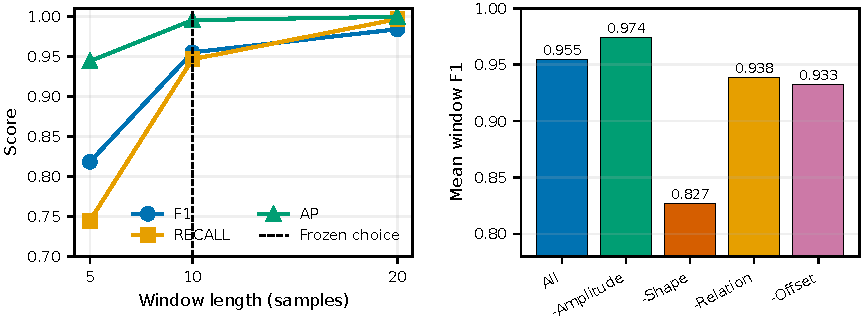
\includegraphics[width=\textwidth]{figures/sensitivity_ablation.pdf}
\caption{Left: window sensitivity for B1; $w=10$ remains the frozen choice. Right: leave-one-feature-group-out audit. Removing shape (S) causes the largest degradation; removing amplitude (A) improves the diagnostic run.}
\label{fig:sensitivity}
\end{figure*}

Counterfactual repair replaces one anomalous channel by its training median. Mean B1 score reductions are 0.0280 for AI0 vibration, 0.0106 for AI1 vibration, and 0.0070 for AI2 current. Group-level repair ranks S (0.0641), A (0.0414), O (0.0389), and R (0.0125). The channel and group analyses answer different questions and need not agree. We label AI0 and S as model evidence, not as the fault location.

\subsection{Stress Tests and Alarm Persistence}

M1 and M2 retain recall 1.0 for all 22 tested anomalous-window perturbations. B1's minimum recall is 0.888 under AI2 dropout, down 0.070 from its fold-0 original recall; M3 falls from 0.988 to 0.530 under the same dropout. Thus, statistical projection models are strongest under the chosen synthetic stresses but fail the normal-regime alarm gate. A deployment can exploit this complementarity by using M1/M2 as diagnostic corroborators without allowing them to directly page operators.

Alarm persistence exposes another trade-off. At $k=1$, mean anomalous-burst detection is 0.988 but the worst normal block produces 20 alarms. At $k=3$, these values are 0.929 and two; at $k=5$, they are 0.894 and one. We retain $k=3$.

\begin{figure*}[t]
\centering
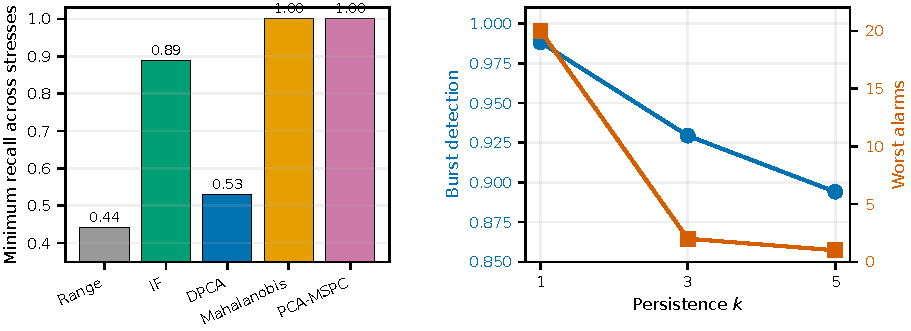
\includegraphics[width=\textwidth]{figures/robustness_persistence.pdf}
\caption{Left: minimum recall over 22 frozen-threshold perturbations. Right: increasing alarm persistence reduces the worst normal-block alarm count but also lowers anomalous-burst detection.}
\label{fig:robustness}
\end{figure*}

\section{Operational Interpretation}

The four-state interface is designed to limit the consequences of non-identifiability. Green continues operation. Yellow-S requests verification of sensor mounting, gain, DAQ configuration, and operating condition before model adaptation. Yellow-F requests repeat measurement under the same condition and equipment inspection. Red combines both evidence types and receives the highest priority, while still avoiding a claim that the model has localized a mechanical root cause.

Out-of-fold normal predictions contain 14,694 Green, 108 Yellow-S, 54 Yellow-F, and 15 Red windows. Median-ensemble anomalous predictions contain 406 Red, 11 Yellow-S, three Yellow-F, and eight Green windows. These counts describe overlapping windows, not independent decisions; the persistence layer remains the operational unit. If AI2 is absent, the stress audit requires a degraded-mode flag and Yellow-S handling rather than silent imputation.

\section{Limitations}

First, normal and anomalous data come from different days, so fault, operation, and acquisition effects are confounded. No method can identify a mechanical cause from these labels alone. Second, there is one anomalous record and no pre-failure onset; we estimate detection on known anomalous operation, not remaining useful life or lead time. Third, stride-one windows overlap by 90\%, so neither fold-level anomaly results nor empirical $p$-values are independent replicates. Our burst audit makes this visible but cannot restore exchangeability. Fourth, 2,000 seconds of normal acquisition are insufficient to certify a low long-run FAR; the Poisson upper bounds remain wide. Fifth, stress tests are synthetic and cover only specified perturbations. Finally, the feature ablation used anomaly labels diagnostically; promoting its best variant without a new held-out fault record would be post-hoc optimization.

Future data collection should span multiple normal loads, sensor remounts, maintenance cycles, and independently occurring failures. A nested protocol could then tune windows and feature groups without reusing the sole fault record, while sequential conformal or online false-discovery control could be evaluated over genuinely continuous operation.

\section{Conclusion}

On a burst-sampled hydraulic pump record, the highest-F1 detector is not the safest alarm policy. SHIFT-Guard couples gap-safe preprocessing, blocked normal validation, normal-only calibration, explicit alarm persistence, and separate shift/fault evidence. This protocol selects Isolation Forest at F1 0.949 and AP 0.994 because it limits every held-out normal block to at most two alarms, rejecting two nominally near-perfect models that produce five. The main scientific result is therefore not a leaderboard number, but a reproducible demonstration that operating-regime robustness, acquisition structure, and evaluation units can change the preferred industrial anomaly detector.

\section*{Impact Statement}

This work aims to reduce missed equipment anomalies and unnecessary inspections. False negatives could permit damage, while false positives could stop production or desensitize operators. The proposed states are decision support, not autonomous shutdown commands, and explanations must not be interpreted as certified root causes. Deployment should include human review, access controls for sensor data, documented degraded modes, and periodic validation on newly collected normal and fault records.

\bibliography{references}
\bibliographystyle{icml2026}

\clearpage
\appendix

\section{Reproducibility Details}

The full pipeline uses Python 3.13.9, NumPy 2.5.1, pandas 2.2.3, and scikit-learn 1.7.2. Raw-file SHA-256 hashes, package versions, the complete configuration, and runtime are stored in the run manifest. Four automated tests verify gap-safe window counts, absence of burst leakage across folds, and empirical calibration behavior. The final prediction table has 15,299 rows and no missing values in fault score, shift score, or their empirical $p$-values.

The machine also contains an AMD Radeon 860M GPU and an AMD NPU, but the installed PyTorch build and ONNX Runtime providers are CPU-only. Because the full statistical experiment completes in under 30 seconds, the artifact uses native CPU execution to avoid adding non-portable accelerator dependencies.

\begin{table}[h]
\caption{Frozen hyperparameters.}
\label{tab:hyper}
\centering
\small
\begin{tabular}{ll}
\toprule
Parameter & Value \\
\midrule
Gap boundary & $>0.5$ s \\
Window / stride & 10 / 1 samples \\
Normal folds & 5 temporal burst blocks \\
Calibration quantile & 0.995 (higher method) \\
Alarm persistence & 3 above / 3 below \\
Isolation Forest & 300 trees, max samples 256 \\
PCA variance & 0.95 \\
B1 seeds & 42, 1337, 2026 \\
\bottomrule
\end{tabular}
\end{table}

\section{Calibration Audit}

For B1 at seed 42, the mean held-out normal fraction with C0 window-level $p\leq0.005$ is approximately 0.00463 across five folds, but fold values range from 0.00177 to 0.00856. Dependence and regime shift explain why matching the nominal level in aggregate is not a coverage certificate. Burst maximum and burst 95th-percentile references contain only about 100 units per calibration fold, giving minimum $p$-values around 0.009--0.010 under \cref{eq:pvalue}; they cannot resolve $\alpha=0.005$. A longer deployment record is required before choosing a burst-level significance level.

\section{Why the Prior LSTM Result Is Excluded}

A prior TensorFlow LSTM encoder-decoder experiment exists for this dataset, but it used a different guide-style split, window length, and threshold rule. Its best recorded configuration obtained F1 0.671 and AP 0.840 after 300 epochs, but direct placement in \cref{tab:main} would imply protocol comparability that does not exist. TensorFlow is unavailable in the native Python 3.13 environment used for the frozen run. We therefore document the result as provenance only and do not count it as a same-protocol candidate.

\section{State Semantics}

\begin{table}[h]
\caption{SHIFT-Guard evidence states and recommended actions.}
\centering
\small
\begin{tabular}{llll}
\toprule
Shift & Fault & State & Action \\
\midrule
Low & Low & Green & Continue; log \\
High & Low & Yellow-S & Check sensor/DAQ/regime \\
Low & High & Yellow-F & Repeat and inspect \\
High & High & Red & Prioritize review \\
\bottomrule
\end{tabular}
\end{table}

\end{document}
